\documentclass{masterthesis-uc2-en}
\usepackage{listings}
\usepackage{color}
\usepackage[caption=false]{subfig}

\definecolor{dkgreen}{rgb}{0,0.6,0}
\definecolor{gray}{rgb}{0.5,0.5,0.5}
\definecolor{mauve}{rgb}{0.58,0,0.82}

\lstset{frame=tbrl,
  language=Python,
  showstringspaces=false,
  columns=flexible,
  numbers=none,
  numberstyle=\tiny\color{gray},
  keywordstyle=\color{blue},
  commentstyle=\color{dkgreen},
  stringstyle=\color{mauve},
  breaklines=true,
  breakatwhitespace=true,
  tabsize=2
}

%% Metadata
\department{Department of Fundamental Computing and its Applications (IFA)}
\specialty{Sciences and Technologies of Information and Communication (STIC)}
\title{Cybersecurity of smart grid infratsructure communication} 
\studentFullnameA{ochetati ilyes chiheb eddine}
\studentFullnameB{kechicheb ahmed}
\supervisorFullnameA{Salim benayoune}
\session{June 2024}

%% Additional commands
%-------------------------------------------------------
% Listings (Source codes) configuration
%-------------------------------------------------------

\definecolor{color-lst-string}{RGB}{166,95,18}
\definecolor{color-lst-annotation}{RGB}{128,128,0}
\definecolor{color-lst-constant}{RGB}{5,133,5}
\definecolor{color-lst-keyword}{RGB}{33,33,255}
\definecolor{color-lst-class}{RGB}{0,112,192}
\definecolor{color-lst-accessor}{RGB}{125,0,84}
\definecolor{color-lst-red}{RGB}{255,0,0}
\definecolor{color-lst-comment}{RGB}{168,166,171}

% XML
\lstdefinelanguage{XML}{
	alsoletter=-.,
	morestring=[b]",
	morecomment=[s]{<?}{?>},
	morecomment=[s]{<!--}{-->},
	morekeywords={
		manifest,application,activity,uses-permission,
	%	...
	},
}

% Java
\lstdefinelanguage{Java}{
	alsoletter=&,
	deletekeywords=SAVE,%	language=Java,
	morestring=[b]',
	morestring=[b]",
	morecomment=[s]{/*}{*/},
	morecomment=[l]{//},
	keywordstyle={[1]\color{color-lst-keyword}},
	morekeywords=[1]{
		super,import,class,interface,void,extends,implements,new,this,null,true,false,return,break,
		if,else,for,while,foreach,switch,case,
		int,long,float,double,boolean,&&,
	},
	keywordstyle={[2]\color{color-lst-class}},
	morekeywords=[2]{
		Bundle,String,Activity,R,View,TextView,Button,List,ArrayList,ViewGroup,Build,Manifest,
%		...
	},
	keywordstyle={[3]\color{color-lst-accessor}},
	morekeywords=[3]{public,private,protected,package},
	keywordstyle={[4]\color{color-lst-annotation}},
	morekeywords=[4]{@Override},
	keywordstyle={[5]\color{color-lst-constant}},
	morekeywords=[5]{
		LENGTH\_LONG,LENGTH\_SHORT,ACTION_CALL,RESULT_OK,
%		...
	},
}

% HTML

% Javascript

% ...

\begin{document}


\frontmatter
	\maketitlepage
	\pagestyle{plain}
	
	\setcitestyle{numbers}
	\hypersetup{citecolor=blue}

	\chapter*{Acknowledgments}
\addcontentsline{toc}{chapter}{Acknowledgments}


%(This section allows you to thank all the people who have participated in the successful development of the end of studies project, and especially when writing your thesis. This \textbf{must not exceed 1~page maximum}.)



We thank ALLAH the Almighty, Great and Merciful for us having given confidence, good health, patience, will and courage to complete this work.

We thank Mr"Salim Benayoune" for his support and commendable effort, for his precious guidance, and assistance during the completion of this work.

We thank our parents who have surrounded us with strength and devoted love ever since we were born.
	\chapter*{Dedication}
\addcontentsline{toc}{chapter}{Dedication}

(In this section, you dedicate this thesis to important people for you. This \textbf{should not also exceed 1~page}.)  % Optional
	
	\addcontentsline{toc}{chapter}{Abstracts}
	\begin{abstractAr}





		تتعرض موثوقية الشبكة الذكية وأمنها لخطر كبير بسبب الاعتماد المتزايد على تقنيات الشبكة الذكية، والتي جلبت نقاط ضعف جديدة تتمثل في التهديدات السيبرانية. العديد من أنظمة كشف التسلل التقليدية \LR{(IDSs)} غير قادرة على اكتشاف معظم هذه التهديدات بسبب التعقيد وبيانات الشبكة الذكية. تقدم هذه الأطروحة نظام كشف التسلل إلى الشبكة القائم على التعلم العميق \LR{(DL-NIDS)} الذي يعالج هذه المشكلة
		
		  تستخدم \LR{NIDS} المستندة إلى \LR{DL} بنية مبتكرة تستخدم الشبكات العصبية التلافيفية \LR{(CNNs)} والشبكات العصبية المتكررة \LR{(RNNs)} لاكتشاف الانحرافات في حركة مرور شبكة الشبكة الذكية. وهذا يشمل الأنماط العادية وكذلك تلك المؤذية.
		
		  ولتقدير أدائها، تم تدريب هذه النماذج على بيانات حركة مرور الشبكة الحقيقية ثم تم اختبارها على مجموعة جديدة من البيانات. وعلى النقيض من أجهزة كشف الهوية التقليدية، هناك تحسن كبير في كل من المتانة ودقة الكشف كما هو موضح في النتائج. كما ثبت أن النظام قادر على اكتشاف مجموعة متنوعة من هجمات DoS وDDoS. ولذلك، فإن هذا البحث يعزز موثوقية وسلامة أنظمة البنية التحتية الحيوية هذه من خلال المساهمة في إيجاد حلول أفضل للأمن السيبراني للشبكات الذكية.
		
		

\end{abstractAr}

\begin{keywordsAr}
	(الشبكة الذكية، الأمن السيبراني، التعلم العميق، هجمات حجب الخدمة، الشبكة العصبية التلافيفية، الذاكرة الطويلة قصيرة المدى)
\end{keywordsAr}

\newpage 
	\begin{abstractEn}
	

	The smart grid's reliability and security are at significant risk due to the increasing reliance on smart grid technologies, which have brought in new vulnerabilities which is cyber threats. Many traditional intrusion detection systems (IDSs) are unable to detect most of these threats because of the complexity and smart grid data.This thesis introduces a deep learning-based network intrusion detection system (DL-NIDS) that tackles this issue

	The DL-based NIDS uses an innovative architecture utilizing convolutional neural networks (CNNs) and recurrent neural networks (RNNs) to discover deviations in smart grid network traffic. This includes normal patterns as well as those that are maleficent.

	To estimate its performance, these models were trained on real life network traffic data then tested on a new set of data. In contrast to conventional IDSs, there is a dramatic improvement in both robustness and detection accuracy as shown by results. The system is also demonstrated to be capable of detecting a variety of DoS and DDoS attacks. Therefore, this research enhances the dependability and safety of such critical infrastructure systems by contributing towards better cybersecurity solutions for smart grids.


\end{abstractEn}

\begin{keywordsEn}
	(smart grid, cybersecurity, deep learning, denial of service attacks, Convolutional neural network , Long short-term memory)
\end{keywordsEn}



\newpage

	%\begin{abstractFr}
%	
%	(Vous insérez ici le résumé du manuscrit en français, dont le nombre de mots \textbf{ne doit pas dépasser 200}.)
%	
%\end{abstractFr}
%
%\begin{keywordsFr}
%	(6 mots clés au maximum doivent être séparés par des virgules ",")
%\end{keywordsFr}




\begin{abstractFr}


La fiabilité et la sécurité du réseau intelligent sont considérablement menacées en raison du recours croissant aux technologies de réseau intelligent, qui ont introduit de nouvelles vulnérabilités que sont les cybermenaces. De nombreux systèmes de détection d'intrusion (IDS) traditionnels sont incapables de détecter la plupart de ces menaces en raison de la complexité et des données des réseaux intelligents. Cette thèse présente un système de détection d'intrusion réseau basé sur l'apprentissage profond (DL-NIDS) qui s'attaque à ce problème.

  Le NIDS basé sur DL utilise une architecture innovante utilisant des réseaux neuronaux convolutifs (CNN) et des réseaux neuronaux récurrents (RNN) pour découvrir les écarts dans le trafic du réseau intelligent. Cela inclut les schémas normaux ainsi que ceux qui sont maléfiques.

  Pour estimer ses performances, ces modèles ont été formés sur des données réelles de trafic réseau puis testés sur un nouvel ensemble de données. Contrairement aux IDS conventionnels, les résultats montrent une amélioration considérable de la robustesse et de la précision de la détection. Le système s’est également révélé capable de détecter diverses attaques DoS et DDoS. Par conséquent, cette recherche améliore la fiabilité et la sécurité de ces systèmes d’infrastructures critiques en contribuant à de meilleures solutions de cybersécurité pour les réseaux intelligents.


  \end{abstractFr}



  \begin{keywordsEn}
	(grille intelligente, cybersécurité, apprentissage profond, attaques par déni de service, réseau neuronal convolutif, mémoire à long terme)
\end{keywordsEn}


	%\clearpage
	
	\tableofcontents
	\listoffigures
	\listoftables
	\listofalgorithms  % Optional

\mainmatter
	\pagestyle{fancy}
	\chapter*{General Introduction} 
\label{chap:introduction} 
\addcontentsline{toc}{chapter}{General Introduction}

(The introduction, which \textbf{must not exceed 3~pages}, consists of the following four sections.)

\section*{Project Background}
(In this section, you describe the context in which your project is being processed.)

\section*{Problem}
(Here, you describe the problem that needs to be solved in the development of your thesis. It comes directly from the theme proposed by your supervisor(s).)

\section*{Proposed Solutions}
(Here, you list the objectives of your thesis study, as well as the solutions you consider to answer the addressed problem.)

In this work, we propose...

\section*{Document Plan}
This thesis is organized as follows: In the first chapter, we...

	\chapter{State of the Art} \label{chap:state_of_the_art}


\section*{Introduction}
Electricity grids, commonly referred to as “grids,” play a vital role in modern energy infrastructure. They facilitate power generation, transmission, distribution, and control. Over time, grids have evolved from localized systems to interconnected networks, adapting to meet increasing demands and technological advancements. These grids contribute significantly to economic and societal progress.

Amidst dynamic changes in the energy landscape, the emergence of the “smart grid” presents transformative possibilities. Leveraging data, automation, and connectivity, smart grids enhance energy management and promote sustainability. In this chapter, we delve into the evolution of grid systems and explore the challenges and opportunities associated with smart grid technology, shaping the future of energy.
\newpage


\section{Definition smart grid}
The Smart Grid is a comprehensive electrical network that employs cutting-edge communication technologies, computational intelligence, and cybersecurity protocols throughout the entire process of generating, transmitting, distributing, and consuming electricity. Its objective is to establish a system that is environmentally friendly, secure, dependable, adaptable, energy-efficient, and environmentally sustainable. While the ultimate vision of the Smart Grid is ambitious, its practical implementation demands careful evaluation of costs, rigorous testing, and validation. Introducing new functionalities can occur autonomously, with each necessitating justification and a reasonable return on investment. The compatibility of open systems facilitates smooth integration into the Smart Grid once the technologies have been validated.\cite{gharavi2011smart}
 The National Institute of Standards and Technology (NIST), operating within the U.S. Department of Commerce, has classified the smart grid into seven distinct domains, as illustrated in Figure 1.1. A concise overview of these domains and their stakeholders is provided in Table 1.2.\cite{gopstein2021nist}
\begin{figure}[h]
	\centering
	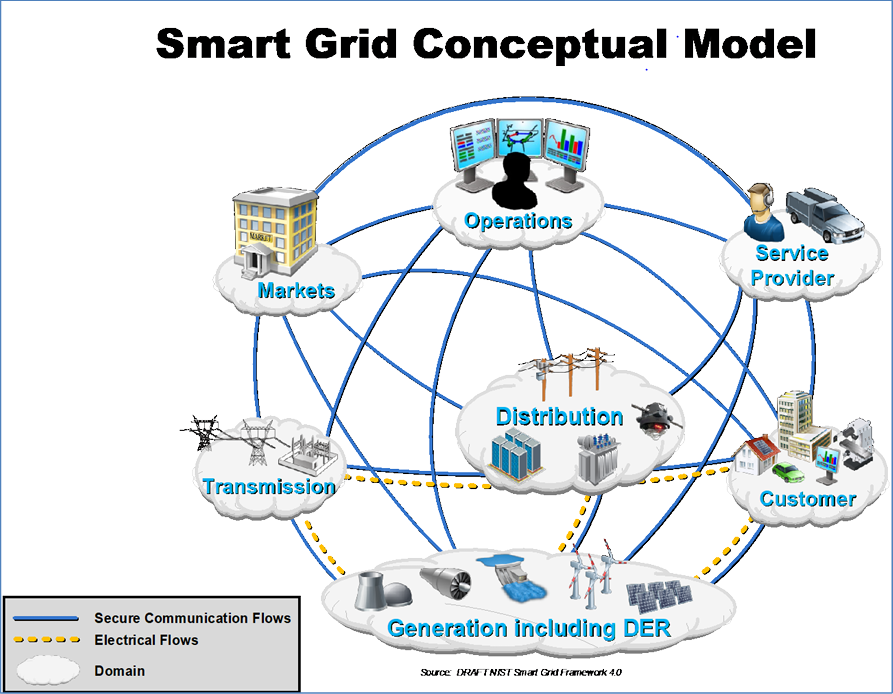
\includegraphics[width=\textwidth]{figures/nist.PNG}
	\caption{The NIST Conceptual Model for SG \cite{gopstein2021nist}}
	% \label{fig:example}
\end{figure}
\begin{table}[h]
    \centering
 %%ffffff
    
% \begin{tabularx}{\textwidth}{|X|X|}
% \hline
% \textbf{Domain} & \textbf{Roles/Services in the Domain} \\
% \hline
% 1 Customer & The end users of electricity. May also generate, store, and manage the use of energy. Traditionally, three customer types are discussed, each with its own sub-domain: residential, commercial, and industrial. \\
% \hline
% 2 Markets & The facilitators and participants in electricity markets and other economic mechanisms used to drive action and optimize system outcomes. \\
% \hline
% 3 Service Provider & The organizations providing services to electrical customers and to utilities. \\
% \hline
% 4 Operations & The managers of the movement of electricity. \\
% \hline
% 5 Generation Including DER & The producers of electricity. May also store energy for later distribution. This domain includes traditional generation sources and distributed energy resources (DER). \\
% \hline
% 6 Transmission & The carriers of high voltage electricity over long distances. May also store and generate electricity. \\
% \hline
% 7 Distribution & The distributors of electricity to and from customers. May also store and generate electricity. \\
% \hline
% \end{tabularx}
\begin{tabular}{|p{0.15\textwidth}|p{0.8\textwidth}|}
    \hline
    \textbf{Domain} & \textbf{Roles/Services in the Domain} \\
    \hline
    1 Customer & The end users of electricity. May also generate, store, and manage the use of energy. Traditionally, three customer types are discussed, each with its own sub-domain: residential, commercial, and industrial. \\
    \hline
    2 Markets & The facilitators and participants in electricity markets and other economic mechanisms used to drive action and optimize system outcomes. \\
    \hline
    3 Service Provider & The organizations providing services to electrical customers and to utilities. \\
    \hline
    4 Operations & The managers of the movement of electricity. \\
    \hline
    5 Generation Including DER & The producers of electricity. May also store energy for later distribution. This domain includes traditional generation sources and distributed energy resources (DER). \\
    \hline
    6 Transmission & The carriers of high voltage electricity over long distances. May also store and generate electricity. \\
    \hline
    7 Distribution & The distributors of electricity to and from customers. May also store and generate electricity. \\
    \hline
    \end{tabular}
    \caption{Domains and their associated roles/services \cite{gopstein2021nist}}
    % \label{table:domains}
\end{table}
\section{Smart grid attributes}
Many smart grid advocates cite some or all of its following attributes as representative of its promise:
\firmlist
\begin{itemize}


\item \textbf{  Efficiency:} Capable of meeting growing consumer demand without the need for additional infrastructure.

\item \textbf{  Flexibility: }Able to accept energy from various sources, including solar and wind, with the same ease as traditional fuels like coal and natural gas. It can integrate new technologies, such as energy storage, as they become commercially viable.

\item \textbf{  Empowering: }Facilitating real-time communication between consumers and utility providers, allowing consumers to adjust their energy usage based on factors like price and environmental concerns.

\item \textbf{  Opportunistic:} Creating new markets and opportunities by leveraging plug-and-play innovations whenever suitable.

\item\textbf{   Focus on Quality:} Able to deliver reliable power without disruptions, ensuring the smooth operation of digital technologies crucial to our economy.

\item \textbf{  Resilience:} Increasingly resistant to cyber attacks and natural disasters through decentralization and the implementation of smart grid security measures.

\item \textbf{  Environmental Sustainability:} Contributing to the mitigation of climate change and offering a viable path towards reducing the environmental impact of electricity generation. \cite{el2014smart}
\end{itemize}


\section{Differences between Traditional grid and Smart grid }
Table 1.1 offers a thorough comparison of the conventional power grid with the smart grid. In contrast to the traditional grid where customers play a passive role, the smart grid actively engages them through bi-directional communication technologies. For instance, rooftop photovoltaic solar panels produce electricity during the day, enabling customers to sell surplus energy back to the grid. At night, these panels continue to power home appliances as usual. Moreover, the smart grid incorporates innovative technologies like distributed generation, electric vehicle charging and discharging, and Flexible Alternating Current Transmission Systems (FACTS) to improve energy distribution and management.\cite{zhang2014smart}
\begin{table}[h]
  
	\caption{Comparison between conventional grid and smart grid \cite{miller2008understanding}}
    

	\begin{tabular}{|p{3cm}|p{6cm}|p{6cm}|}
	\hline
	Aspects & Conventional Grid & Smart Grid \\
	\hline
	Interaction between Grid and Customers & Customers passively accept service from grid & Customers participation on the grid action \\
	\hline
	Renewable Energy Integration & Having trouble with renewable penetration & Integration with renewable resources enhancement \\
	\hline
	Options for Customers & No choice for customer, monopoly market & With digital market trading, PHEV, introduce bids and competition, more choice for customer \\
	\hline
	Options on Power Quality (PQ) & No choice on power quality, no price plan options for consumers & Power quality levels for different consumers \\
	\hline
	System Operation & Ageing power assets, no efficient operation & Assets operating optimization, less power loss \\
	\hline
	Protection & Only rely on protection devices, fault detect manually & Have capability of self-healing, less damage affected by fault \\
	\hline
	Reliability and Security & Susceptible to physical and cyber attack & More reliable for national security and human safety \\
	\hline
	\end{tabular}

	\label{tab:my_label}
\end{table}


\section{Components of the Smart Grid }  

\subsection{Smart Meters}
The interplay between smart meters and smart grids is depicted in Figure 1.1. From the perspective of the smart grid, the applications primarily revolve around leveraging smart meters to facilitate the coordination of various electrical devices, thereby achieving a dependable power system. Simultaneously, these applications strive to enhance the performance and efficiency of smart metering. These objectives align with the defining characteristics of smart grids, which drive the advancement of smart meter technologies.\cite{chen2023control}
\begin{figure}[h]
	\centering
	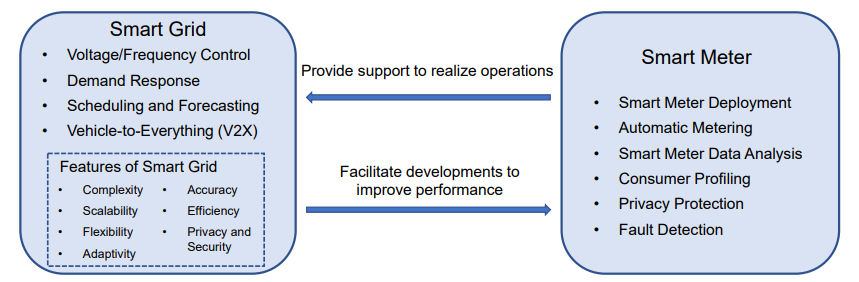
\includegraphics[width=\textwidth]{figures/SmartMeter.PNG}
	\caption{Applications from smart grid and smart meter perspectives. \cite{chen2023control}}
	\label{fig:example}
\end{figure}
\subsection{Advanced Distribution Management Systems }
An ADMS is a software platform designed to support the comprehensive suite of tasks related to managing and optimizing the distribution of electricity. It encompasses functions that automate outage recovery and enhance the effectiveness of the distribution grid. These functions being developed for electric utilities include fault location, isolation, and restoration; optimization of voltage and reactive power; energy conservation through voltage reduction; management of peak demand; as well as support for microgrids and electric vehicles \cite{avazov2016advanced}.

% \firmlist
% \begin{itemize}


% \item \textbf{ Optimizing Power Flow:} ADMS dynamically adjusts power distribution to ensure efficient energy transfer across the grid.

% \item \textbf{  Real-Time Monitoring: }They keep a vigilant eye on the grid, promptly detecting issues like outages.

% \item \textbf{  Rerouting Electricity: }When problems arise, ADMS reroutes electricity to minimize disruptions.

% \end{itemize}
\subsection{Communication Infrastructure}
\subsection{Smart Appliances and Devices}
\subsection{Renewable Energy Integration}

\section{Benefits of Smart Grid}  
\subsection{Increased Efficiency}
\subsection{Improved Reliability}
\subsection{Sustainability and Environmental Benefits}
\subsection{Cost Savings}
\subsection{Consumer Empowerment}
\section{Challenges and Considerations }  
\subsection{Cybersecurity}
Without a shred of doubt, cybersecurity stands out as one of the foremost and intricate challenges confronting IoT devices. Sensors, devices, and networks connected to the internet are persistent targets for various online threats like probing, espionage, ransomware, theft, and potential destruction. Considering that an IoT-driven smart grid can encompass potentially millions of interconnected nodes spread across extensive geographic regions, it emerges as the most susceptible to substantial cyber assaults. Consequently, a cyber-attack on such a system would have devastating consequences, leading to significant financial losses and potentially bringing entire countries to a standstill. The diagram in Figure 1.3 illustrates the number of articles reviewed per year of publication and smart grids impacted by cyber-attacks. Hence, security stands as a major hurdle in both the deployment and operation of IoT-based smart grid networks.\cite{kimani2019cyber}.
\begin{figure}[h]
	\centering
	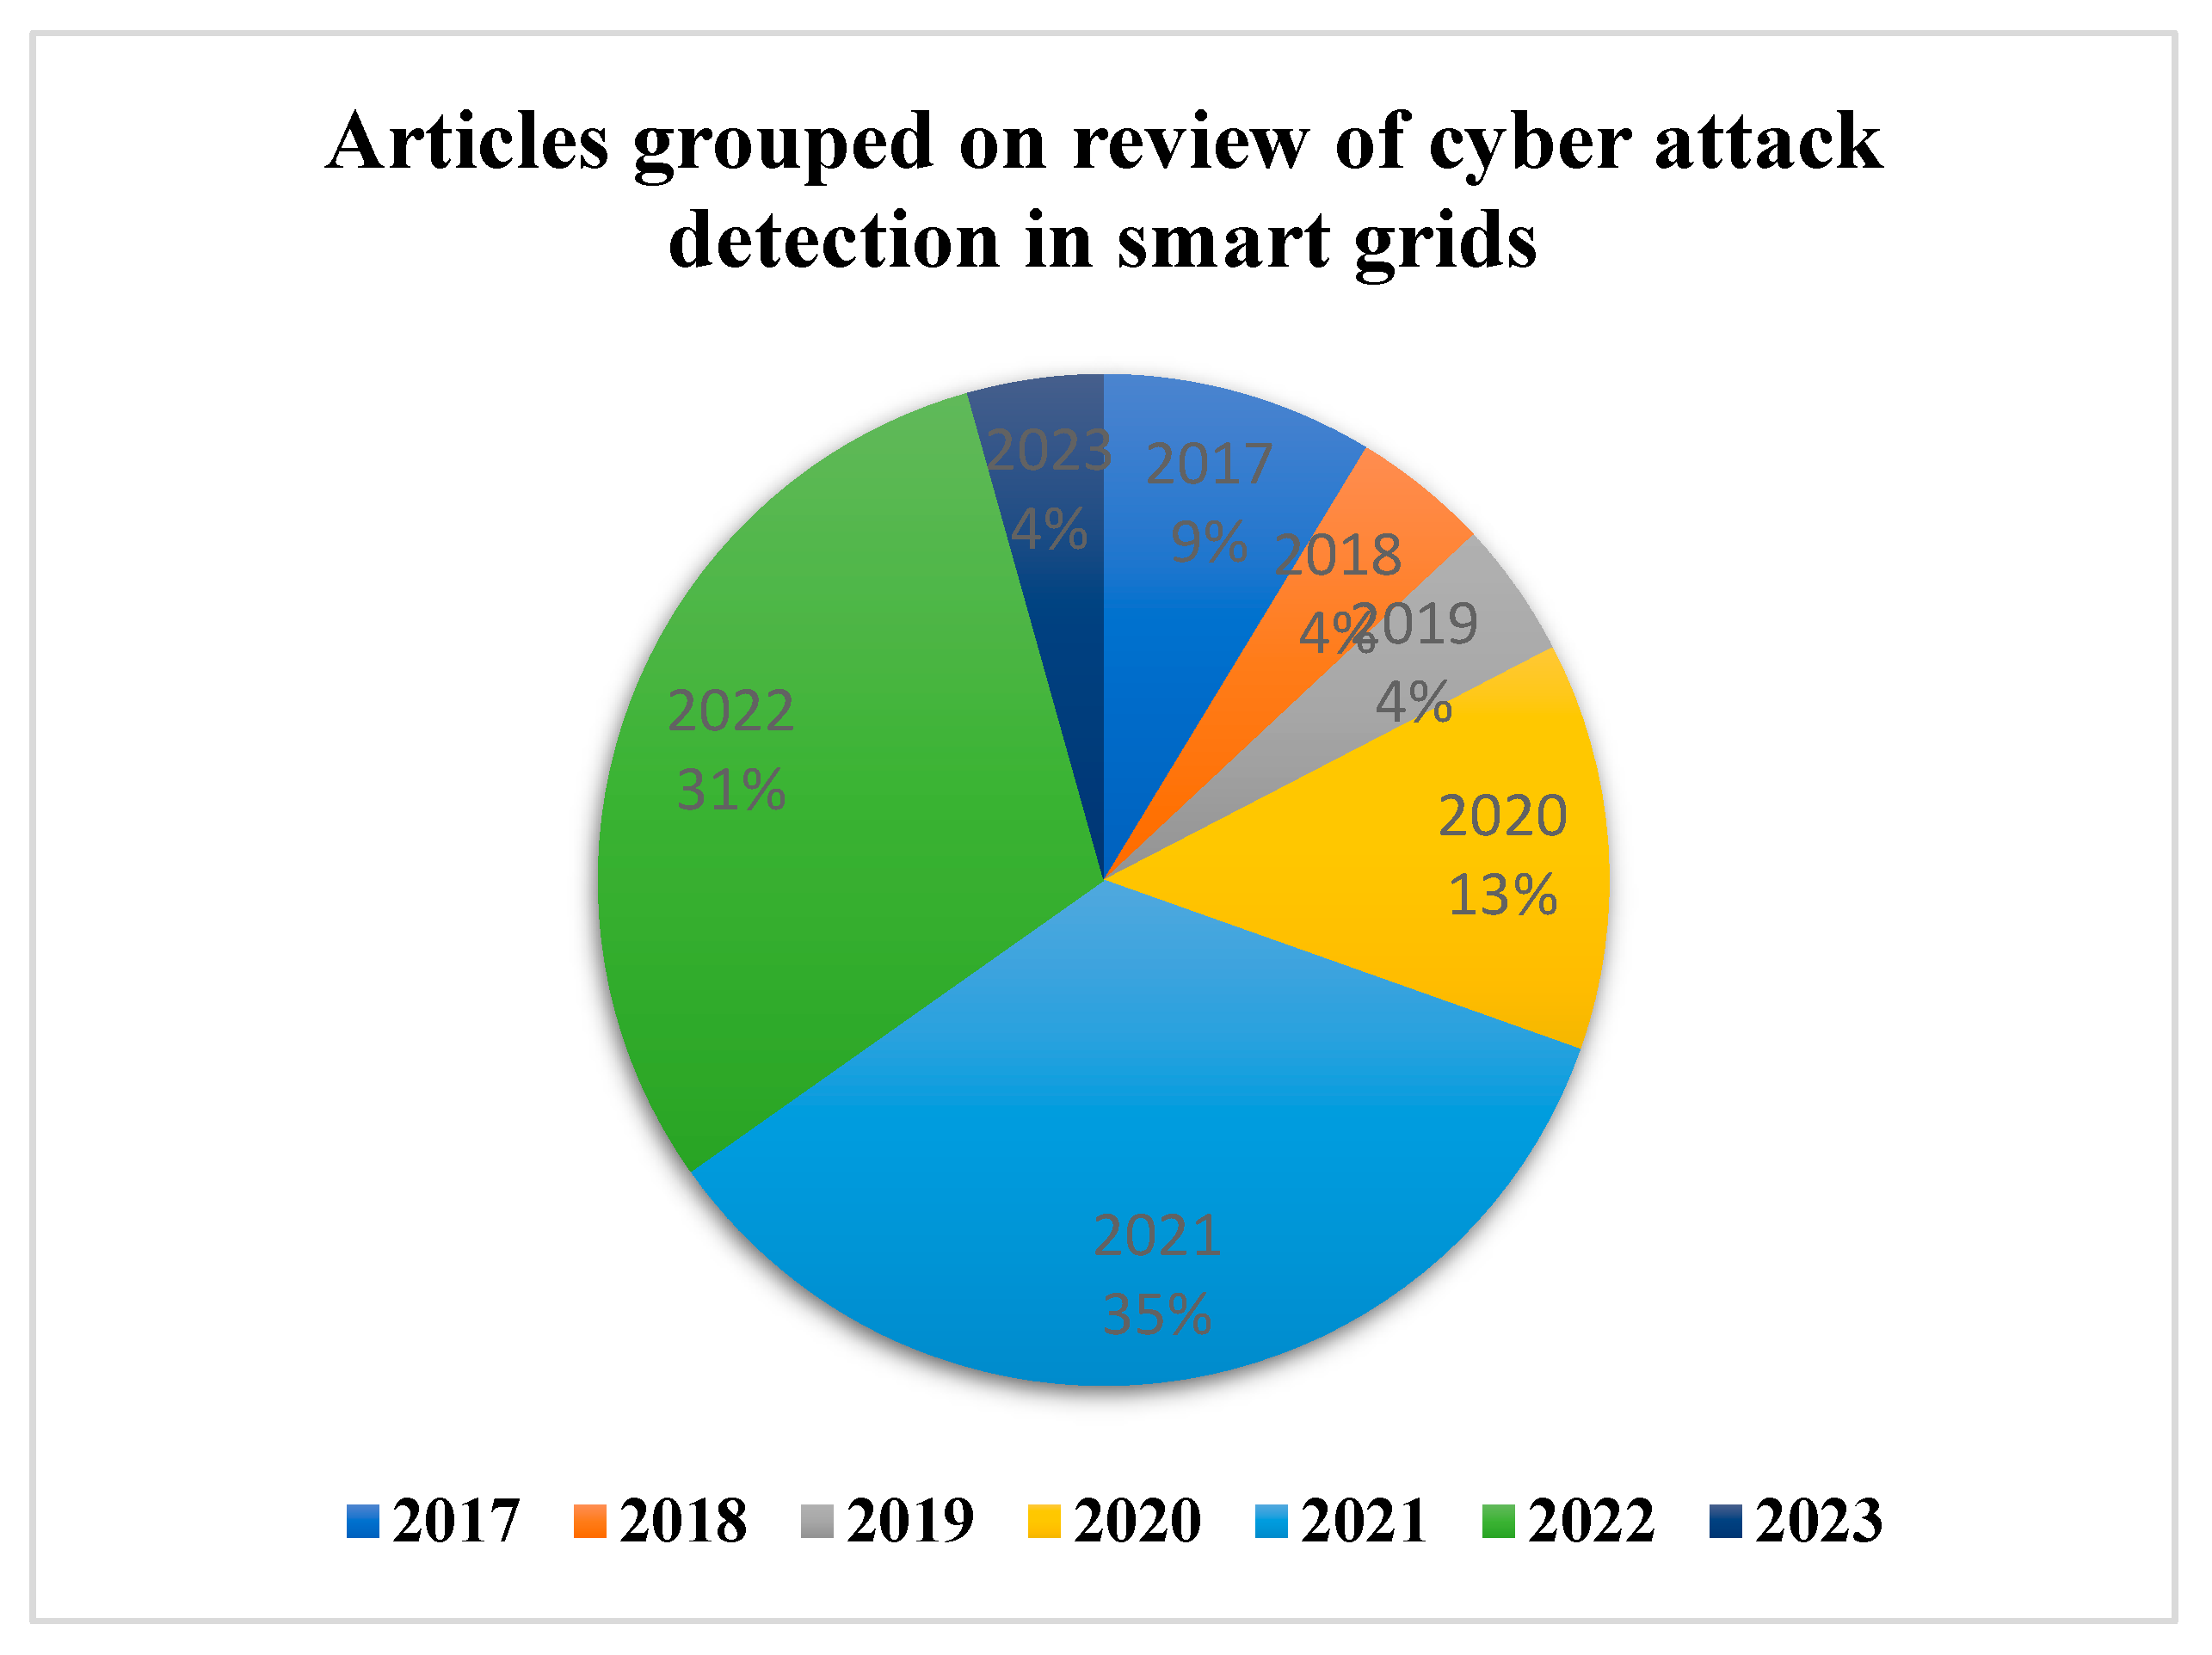
\includegraphics[width=15cm]{figures/attack.png}
	\caption{Estimate: cyber attacks will increase exponentially \cite{mdpi-link}}
	% \label{fig:example}
\end{figure}

\subsection{Data Privacy}
\subsection{Cost of Implementation:}
\subsection{Regulatory Frameworks}
\subsection{Public Awareness and Education}
\section{The Future of Smart Grids }  
\subsection{Distributed Generation}
\subsection{Energy Storage}
\newpage
\section*{Conclusion}
The smart grid revolution is not a destination, but a continuous journey towards a more efficient, reliable, and sustainable energy future. While challenges exist, the potential benefits of the smart grid are undeniable. By embracing innovation, fostering collaboration, and empowering consumers, we can unlock the full potential of this transformative technology.

A smarter grid paves the way for a future where clean energy sources like solar and wind power are seamlessly integrated, homes and businesses actively participate in energy management, and power outages become a rarity. It's a future where we have a more secure and sustainable energy infrastructure for generations to come.

Let's continue exploring the exciting world of smart grids and work together to build a brighter energy future for all.
	




\chapter{Implementation} \label{chap:Implementation}
\section*{Introdution}
%% incomplete
%In this chapter, we will put into practice our proposed approach which is a deep learning model of an IDS that utilises the LSTM algorithm of deep learninglearning

%in the previous chapter in order to test its feasibility and evaluate the results in a study of cases. The objective is to measure the degree of success of our approach. To do this, We will start by proposing a specific 
%XXXXXXX (our specifics)
%which will improve the detection accuracy in smart grid networks

In this chapter, we present our contributions towards the deep learning-based intrusion detection system for the smart grid. due to the fact that smart grid communication requires connecting to the internet, smart grid components now have a new weakness which is cyber-threat. In order to counter this issue, we suggest a deep learning method that utilizes Convolutional Neural Networks (CNNs) and Long Short-Term Memory (LSTM) which is a specific type of Recurrent Neural Network (RNN) to enhance the precision and efficiency of identifying intrusions within the smart grid communication infrastructure.
% mention DoS and DDoS here





\section{Theoretical Proposal}

\subsection{Project Description}
the proposed system for the project is a network intrusion detection system based on deep learning that will depend on either CNN or LSTM as a learning algorithme. This project mainly aims at designing and implementing said system that can detect cyber threats in Smart Grid Communication Infrastructure effectively.To capture both spatial and temporal features of network traffic data, the proposed system will use either CNN or LSTM architectures to identify complex and sophisticated attack patterns that would threaten the smart grid functionality.
Our deep learning based network intrusion detection system will be mainly focused on denial of service attacks (DoS) and distributed denial of service attacks (DDoS).

\subsection{Project Design and architecture}
Building any machine learning or deep learning model usually involves several important steps, as shown in Figure  \ref{fig:DL-creation}.


First, we need to collect data that is relevant to the function of the model we want to train, which we will then need to preprocess, which entails clearning, encoding, augmenting, and standardising the data to prepare it for the training phase.


The next step is to select a learning algorithm, the proper optimizer, a loss function, and the evaluation metrics that we will use to train our model.


The model is then trained on the cleaned data, and this is where we feed the trained model new data it has not yet seen before and get the results and predictions on the new data.


The next and final step is the validation step, in which we get the prediction results and evaluate the model accuracy, recall, and f1-score.

\begin{figure}[h]
	\centering
	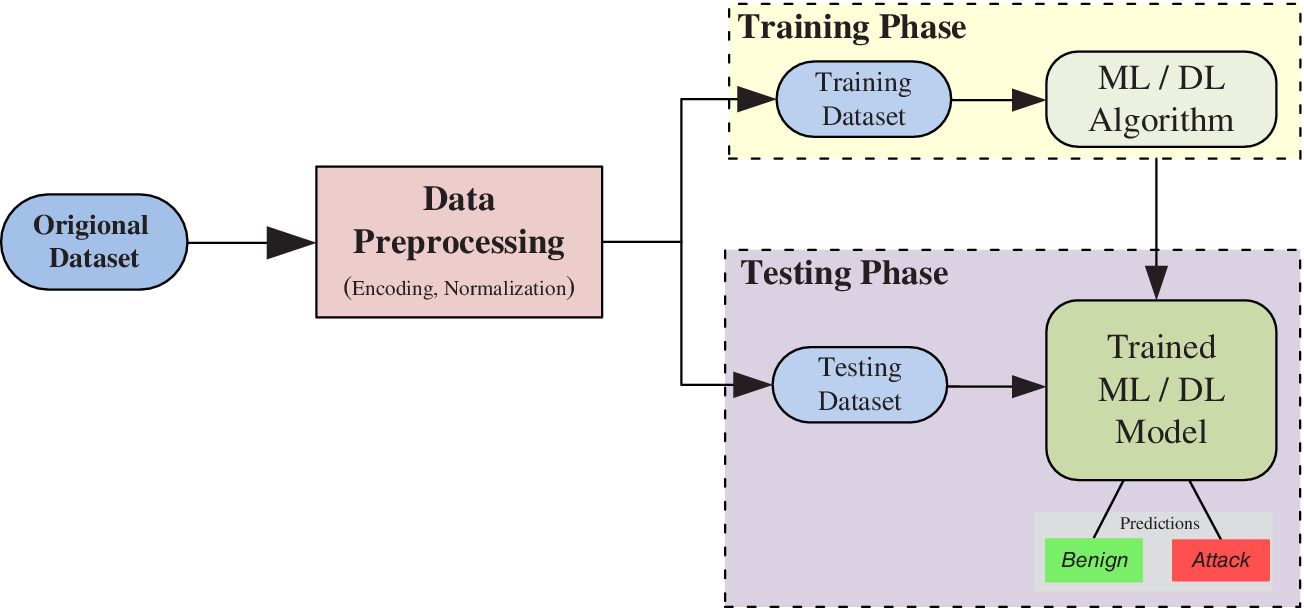
\includegraphics[width=400px]{figures/DL_creation.jpg}
	\caption{deep learning model creation}
	\label{fig:DL-creation}
\end{figure}









\subsection{Deep learning Models architecture}
Detecting cyber threats to the smart grid functionality and safety is crucial a task which needs high accuryacy of detection that's why we opted to  we choose two deep learning algorithms for intrusion detection which are CNN and LSTM



%########################			########################################
%########################			########################################
%########################			########################################
%########################			########################################
%########################			########################################



\subsubsection{CNN model}
Convolutional Neural Networks (CNNs) are a highly-specific deep learning algorithm meant to analyze spatialy structured input data, like images and grid structured data. These are derived from the visual cortex of human beings and are good at image recognition, object detection and image segmentation among others. CNNs work by carrying out convolutional layers in order to capture local characteristics, pooling layers in order to reduce spatial dimensions and fully connected layers for predictions. They can be trained on labeled data and have proved very effective in several applications like face recognition, medical imaging analysis as well as self-driving cars.\cite{CNN}

Note: will expande on this later

% add graph
%talk about layers maybe





%########################			########################################
%########################			########################################
%########################			########################################
%########################			########################################
%########################			########################################
%########################			########################################





\subsubsection{LSTM model}
Long Short-Term Memory (LSTM) is a type of Recurrent Neural Network (RNN) that was developed by Hochreiter and Schmidhuber; LSTM is different from RNNs because it can forecast sequences and study long-term dependency patterns from the provided data. What makes LSTMs unique is their ability to learn order dependency patterns which is critical in solving complex problems like speech recognition and machine translation.
LSTM address the weakness of traditional RNN which is the unability to learn any long term patterns which it solves by introducing a memory cell, LSTM is controlled with Three gates control: input gate, forget gate, output gate.These gates determine what information to add, remove, and output from the memory cell and hence enable LSTM networks to learn long-term dependency patterns. \cite{lstm}

Note: will expande on this later

% add graph
%talk about layers maybe








































































































\section{Implementation and Experiments}





\subsection{Development tools used}
\subsubsection{Development environment}
training deep learning models requires a high performance PC due to the fact that these models require high computational resources to process large datasets and intricate neural networks.  With complex calculations and huge amounts of data. One of the reasons why having a powerful PC with a powerful GPU is important during the training process is that it can significantly shorten the time needed for the training, as well as reduce computational resources. a sufficient quantity of memory (RAM) is also needed to load big datasets, and fast storage devices like SSDs are vital in handling data-intensive nature of deep learning tasks.





\begin{itemize}
	\item jupyter notebook: is an open source web application or a vscode extension that facilitates the creation and sharing of segmented documents that contains blocks of interactive code, text and data visualations, it is mostly used for data science, machine learning and scientific computing, it supports a wide range of programming languages like python, R, scala and julia, it can also display some text formats like markdown, Latex and HTML.
	\item VScode: Visual Studio Code (VS Code) is an open-source source-code editor developed by Microsoft for Windows, Linux, macOS, and web browsers. It is a popular choice among developers due to its extensive features like code highlighting, debugging, code completion, and the ability to extend its original functionality with 3rd-party extensions and extensibility. It also offers Git integration out of the box.
\end{itemize}





\subsubsection{programming languages}
The programming language we mainly used is Python 3, important aspect of Python lies in its being more than just an object-oriented programming language because it supports other programming paradigms, which are procedural and functional programming making it flexible when choosing the desired approach. It has user-friendly syntax making it easy to digest even for beginner, This has led to the rise of Python's ecosystem fostered by active community coupled with simplicity behind coding style making it easily accessible by almost everyone. To further improve its capability and functionality, python boast a wide range of third party packages that can easily be installed through Python package manager called pip. Python was created in 1991 by Guido van Rossum. A major landmark came in 2008 with the development of python3 which introduced several improvements and enhancements to the language thereby cementing its place as a valuable flexible programming tool on earth today. \cite{python}

libraries that are used for the development:

\begin{itemize}
	\item NumPy: NumPy is the primary array programming library for the Python language, with an essential role in research analysis pipelines across diverse fields such as physics, chemistry, astronomy, geoscience, biology, psychology, and more. The NumPy array is an efficient data structure that stores and accesses multidimensional arrays (tensors), enabling a wide variety of scientific computation. NumPy was initially developed by students, faculty and researchers to provide an advanced, open-source array programming library for Python, with a sense of building something consequential together for the benefit of many others. \cite{python}



	\item Pandas: Pandas is a Python open source program meant for data management and analysis, it was started in 2008 by AQR Capital Management. It went public in late 2009 and has an active community of contributors. Some of the most important features associated with pandas are fast and efficient DataFrame object for data manipulation with integrated indexing, tools for reading and writing data between in-memory data structures and different formats, time series functionality like date range generation, frequency conversion, moving window statistics, and date shifting and highly optimized performance with critical code paths written in Cython or C. \cite{pandas}
	

	
	\item Matplotlib: Matplotlib is a 2D plotting library for Python which can produce publication quality plots, used in application development, interactive scripting and image creation on all operating system and user interface platforms. The author of Matplotlib John D. Hunter began using Python in 2001 and was initially frustrated at the lack of a powerful graphics environment like MATLAB's. He then developed Matplotlib to satisfy his needs, focusing initially on embedding it in a GUI for his ECoG application and then gradually adding support for other features like high-quality raster and vector output, support for mathematical expressions, and interactive use from the shell.\cite{plot}


	\item Seaborn: Seaborn is a python library for making statistical graphics, Seaborn is a high-level interface to Matplotlib and compatible with Pandas's data structures. Seaborn can provide the data with a dataset alongside plot specifications and automatically maps the values onto visual attributes such as color, size or style; internally seaborn performs the relevant statistical transformations and finally adds axis labels as well as legends for the plots. Many Seaborn functions can generate multi-panel figures for comparing different subsets of data or variable pairings within a dataset. By allowing quick prototyping and exploratory analysis of data in single-function calls with just a few arguments, Seaborn can be used throughout the scientific project cycle.  \cite{seaborn}
		

	\item scikit-learn: Sckit-learn is a Python library that provides various machine learning algorithms for medium-scale supervised and unsupervised problems. It focuses on making things easy, having good performance, documentation and remaining consistent in it's APIs. Scikit-learn depends on scientific Python ecosystem libraries such as NumPy and SciPy, and uses Cython to blend C/C++ with Python for improved performance. This lightweight software has few requirements and can be obtained by anyone without any major legal challenges since it is distributed under a simplified BSD license. It provides solid implementations of Machine Learning algorithms, documentation and community driven development, scikit-learn also includes some nice implementations of different algorithms outperforming other popular python ML libraries in many instances including SVMs, Lasso, Elastic Net, k-Nearest Neighbors, PCA, k-Means and some other algorithms.\cite{scikit-learn}


	\item TensorFlow: TensorFlow is a free and open-source software library for machine learning and artificial intelligence. It gives you more flexibility and control the some of the other machine learning frameworks with features such as the Keras Functional API and the Sub-Classification API model to build complex neural network topologies. it offers fast execution for fast debugging and simple prototyping.\cite{tf}
	

	\item Keras: Keras is an open-source library that provides a Python interface for artificial neural networks. Keras was first independent software, then it was integrated into TensorFlow library, and later started supporting others like AJX and PyTorch.\cite{keras}




	

\end{itemize}






%################################################################
%################################################################
%################################################################
%################################################################
%################################################################
%################################################################
%################################################################
%################################################################
%################################################################
%################################################################
%################################################################
%################################################################
%################################################################
%################################################################
%################################################################











\subsection{Dataset}\label{Dataset}
The IDS 2018 dataset is the data set used for this project, this dataset is a comprehensive and realistic dataset for intrusion detection systems. it was created through a collaboration effort between the Communications Security Establishment (CSE) and the Canadian Institute for Cybersecurity (CIC). It includes a few types of attacks such as Brute-force, Botnet, DoS, DDoS and Web attacks, also network infiltration from within all of which are a common attack on smart grid systems. This resulted in 16,233,002 traffic samples which were collected over 10 days from ten real networks, an unusual feature of this data set is its imbalance in benign to malicious ratio of cases. The CICFlowMeter-V3 generates 80 features extracted from the network traffic which describe various intrusions along with abstract distribution models for applications, protocols or even lower level networking entities. Researchers widely employ this dataset to analyze their IDS performance in different research works while others use it to build advanced IDS models. This dataset is not specific to smart grid activity but it is a generalized dataset that includes generalized network traffic which would be the same in a smart grid.




\subsection{Data preprocessing}
Data preprocessing is a crucial step, and the first step in training a machine learning model is data preprocessing. It involves cleaning, transforming, and organising the dataset before it can be utilised by the machine learning algorithms. Data preprocessing entails improving dataset quality by addressing issues such as missing values, invalid values, and inconsistencies. Data preprocessing techniques include cleaning the data to get rid of errors, normalising the data so that features have the same scale, and feature engineering, which will result in new informative variables, augmenting the data, and resampling it to avoid bias in our model. Preparing the data effectively ensures that machine learning models can accurately learn patterns, increasing their performance and, hence, more accurate results.



\subsubsection{importing data}
First we load the data with Pandas library, and since our dataset is split into 10 files, we load the files which include the data related to DoS and DDoS attacks and we merge the data into the same variable for easier preprocessing while deleting the old variable to evoid uselessly fillig the memory, we also remove unneeded column from one of the dataset files

\lstinputlisting[language=Python]{listings/loading_data.py}

the total amount of data loaded is about 11 million rows with 80 columns all of which is either benign or DoS/DDoS traffic with a total size of 6.6 GB.

\begin{figure}[h]
	\centering
	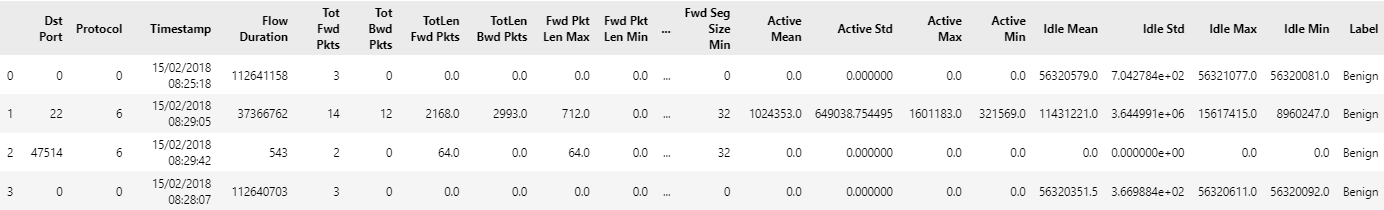
\includegraphics[width=400px]{figures/data_example.png}
	\caption{data sample}
	\label{fig:datasample}
\end{figure}

as we can see in the Figure \ref{fig:unbalanced_data} and Table \ref{tab:unbalanced_data_table} below, the data is unbalnced, but we will fix that later in the data preprocessing phase, specifically in the data augmentation phase.

\begin{figure}[h]
	\centering
	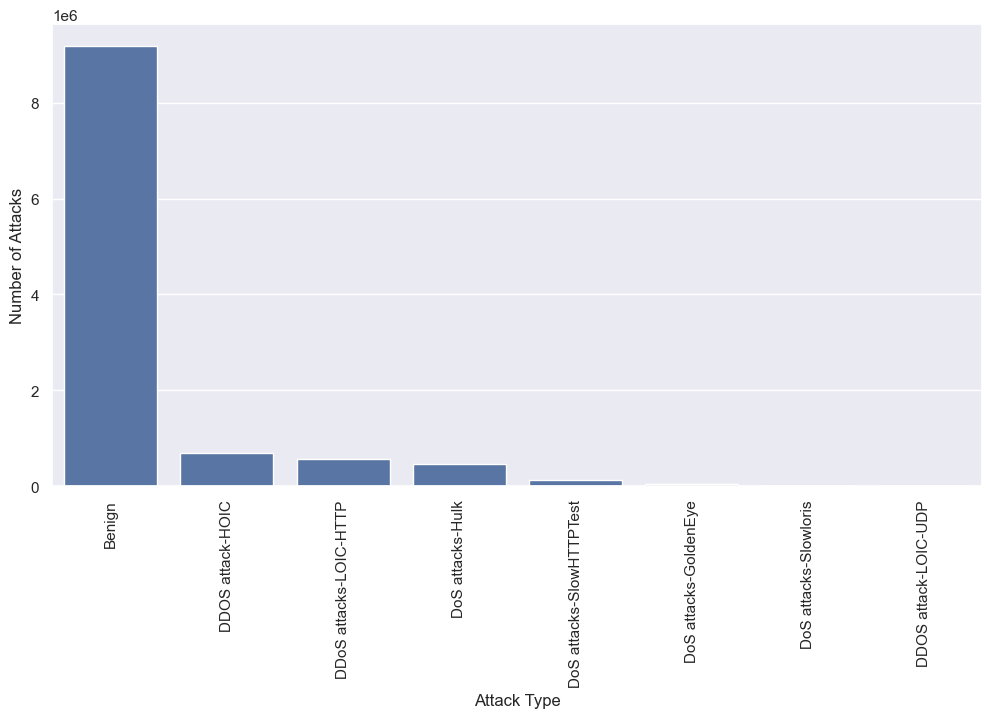
\includegraphics[width=400px]{figures/unbalanced_data.png}
	\caption{data sample}
	\label{fig:unbalanced_data}
\end{figure}

\begin{table}[h]
	\centering
	\caption{the number of occurrence for each traffic type}
	\begin{tabular}{|p{6cm}|p{6cm}|}

\hline activity type & number of ocurences \\
\hline Benign & 9176239 \\
\hline DDOS attack-HOIC & 686012 \\
\hline DDoS attacks-LOIC-HTTP & 576191 \\
\hline DoS attacks-Hulk & 461912 \\
\hline DoS attacks-SlowHTTPTest & 139890 \\
\hline DoS attacks-GoldenEye & 41508 \\
\hline DoS attacks-Slowloris & 10990 \\
\hline DDOS attack-LOIC-UDP & 1730 \\
\hline

\end{tabular}

	\label{tab:unbalanced_data_table} 
\end{table}


\newpage

\subsubsection{Cleaning data}
To clean our data we must first find and remove unwanted data like missing values, null values, duplicate rows and unneeded columns or features.


\firmlist
\begin{itemize}
	\item finding and cleaning missing values: First we identify the columns that contain null values, in a our dataset by identifying columns with missing values,after which we decide to eliminat the rows containing null values, in a Dataset. The objective of this step is to eliminate missing data to ensure quality and consistency Data for the model training.
	\lstinputlisting[language=Python]{listings/cleaning_nulls.py}
	\item removing duplicate rows: we also remove duplicate rows for a better quality dataset and to avoid bias in our model.
	\lstinputlisting[language=Python]{listings/cleaning_dups.py}
\end{itemize}






\subsubsection{Encoding the categorical variables}
The LabelEncoder assigns a unique integer to each categorical value which is the label in our case which is the traffic type(benign or attack), which which allows them to be represented in a numerical form. This makes it easier to use of these variables in machine learning algorithms, as they can handle numerical values better.

\lstinputlisting[language=Python]{listings/encoding_cat_var.py}






\subsubsection{Augmenting the data}
As we have stated before in section \ref{Dataset} that our dataset is unbalanced in the distribution between benign and malicious activity which is a bad thing because it will introduce bias, overfitting and poor prediction performance to our model.







In this step we will resample our dataset to get a better 1:1 ration between our different categorical variables (benign and other attack types).

\lstinputlisting[language=Python]{listings/resample.py}

the python code snippet uses the resample function from scikit-learn, it does the resampling we need to make our dataset balanced 

\begin{itemize}
	\item data x: all of those variables are our data which has been cleaned and separated according to the previously encoded categorical variables.
	\item n samples: is the number of rows for each attack types, in this case we used 20000 rows.
	\item random state: this is the resampling seed, by using the same seed number we can ensure that we always get the same results.
	\item replace: replace decides whether or not the samples can be selected multiple times.
\end{itemize}



% change to pie and change colors
\begin{figure}[h]
	\centering
	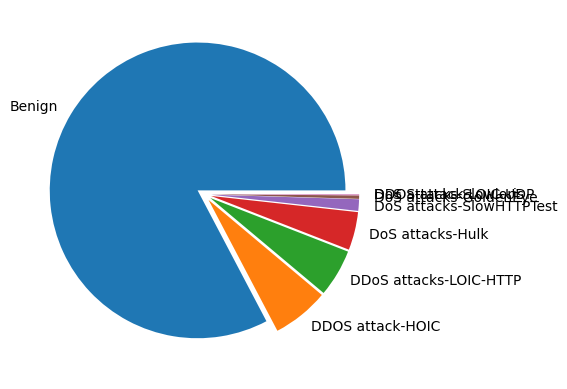
\includegraphics[width=200px]{figures/unbalanced_donut.png}
	\caption{Before data augmentation}
	\label{fig:datasample}
\end{figure}
\begin{figure}[h]
	\centering
	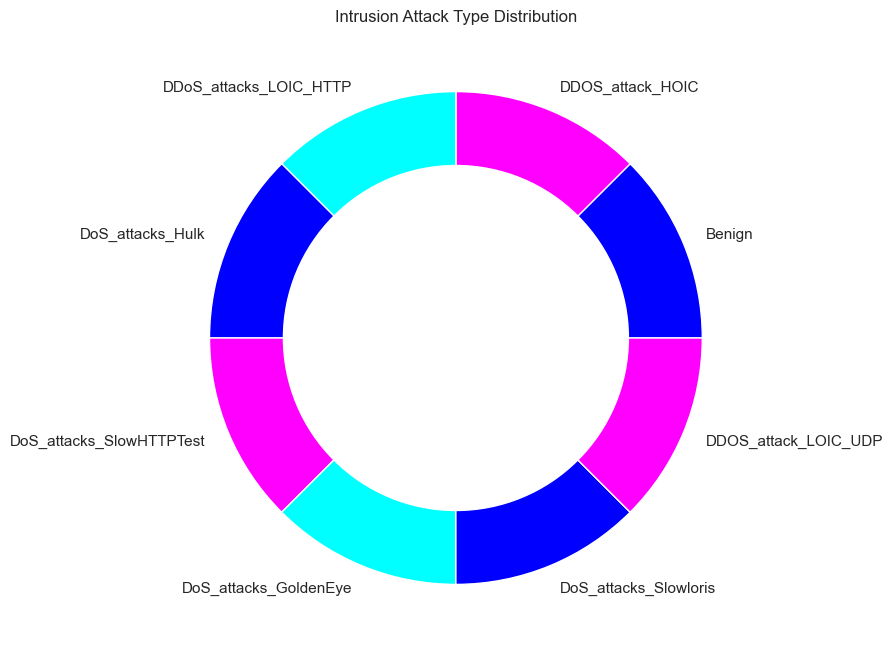
\includegraphics[width=200px]{figures/balanced_donut.png}
	\caption{After data augmentation}
	\label{fig:datasample}
\end{figure}

those resampled variables are then merged and are fed to the deep learning model for training.
% this part's format is broken the pdf file





\subsubsection{splitting the data for the deep learning model}
%maybe add smething here idk
In this step we split our data into 2 sets:
\begin{itemize}
	\item training data: 90\% of the total dataset
	\item testing data 10\% of the total dataset
\end{itemize}
\lstinputlisting[language=Python]{listings/data_split.py}
















%##############################################################
%##############################################################
%##############################################################
%##############################################################
%##############################################################
%##############################################################
%##############################################################
%##############################################################
%##############################################################
%##############################################################
%##############################################################
%##############################################################
%##############################################################
%##############################################################





\subsection{Deep learning models implementation}




\subsubsection{CNN model}
% something here
We built a deep learning model that uses CNN as a learning algorithm with 64 filters, ReLU as the activation function in Python


CNN model summary
\lstinputlisting[language=Python]{listings/CNN_model.py}

% say something here
deep learning model creation:
\firmlist
\begin{itemize}
	\item Sequential(): Creates a Sequential model which is a linear stack of layers.
	\item Conv1D(): adds one dimensional convolutional layer to the model, sets the feature filter and the activation function
	\item MaxPooling1D(): adds one dimensional pooling layer to the model, which is used to reduce the spatial dimensions of the data 
	\item Flatten(): used to convert the multidimensional output of the previous layers into a 1D vector
	\item Dense(): a fully connected layer used to do the classification tasks
	\item BatchNormalization(): used to normalize the data between different layers, it helps improve the model's performance
	\item compile(): used to configure the model, it can set the following parameters:
		\firmlist
		\begin{itemize}
			\item loss function: categorical crossentropy is used to compute the cross-entropy loss between the true class distribution and the predicted class distribution
			\item optimizer: adam adapts the learning rate for each parameter individually making it effective for fast convergence and robustness.
			\item metrics: accuracy is the precision of the predicion as a ratio of correct prediction to the total number of predictions which is a measure of the overall performance of the model. 
		\end{itemize}
\end{itemize}

we also get a summary of the created model, this summary describes the arrangement of the model layers, the number of parameters of each layer, the output shape of each layer and the number of trainable and non-trainable parameters


\newpage

\begin{figure}[h]
	\centering
	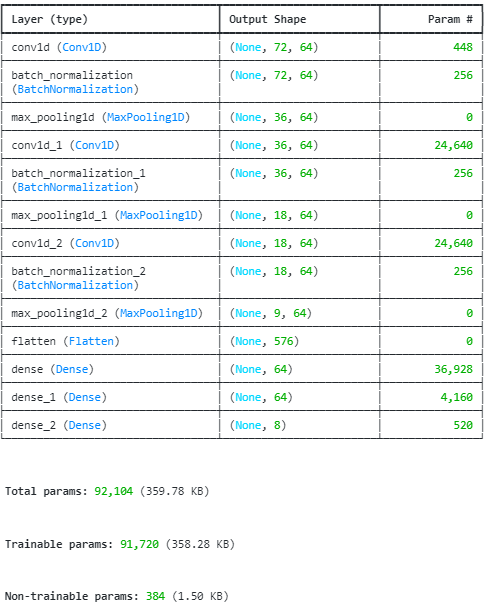
\includegraphics[width=300px]{figures/CNN_model_summary.png}
	\caption{CNN model summary}
	\label{fig:test}
\end{figure}

% add graph
% reùove this title and continue

Next step is starting the model training with 30 epochs, 32 batch sier and the validation data which is the test data we split from the original dataset earlier

\lstinputlisting[language=Python]{listings/CNN_training.py}








%##############################################################
%##############################################################
%##############################################################
%##############################################################
%##############################################################
%##############################################################
%##############################################################
%##############################################################
%##############################################################
%##############################################################
%##############################################################
%##############################################################
%##############################################################
%##############################################################






\subsubsection{LSTM model}
% say something
The LSTM mode implementations is very similar to the CNN implementation with only a few challenges, with those changes being that CNN uses Conv1D() to create it's one dimensional convolutional layer, while LSTM uses LSTM() function to add it's layers 

\lstinputlisting[language=Python]{listings/LSTM_model.py}




we get a model summary for the LSTM model as well


\begin{figure}[h]
	\centering
	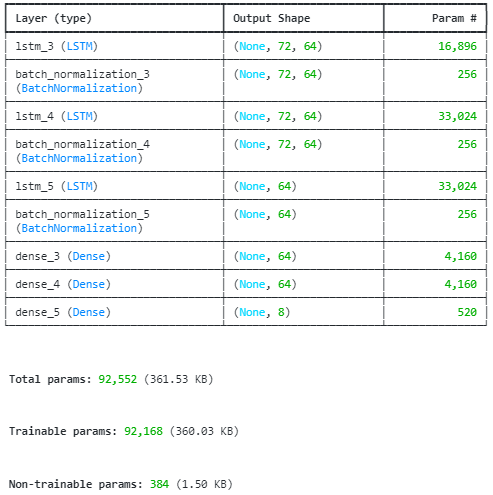
\includegraphics[width=400px]{figures/LSTM_model_summary.png}
	\caption{LSTM model summary}
	\label{fig:test}
\end{figure}













\subsection{Results}
In this we will compile the data from our models evaluation on the test data with both the CNN and the LSTM models, the metrics that we use for evaluation are mainly the detection accuracy and loss rate, we will also be looking at other mertics like
some criteria of evaluation are:

\begin{itemize}
	\item Accuracy: Accuracy measures the overall correctness of a model's predictions. It is calculated as (TP + TN) / (TP + TN + FP + FN). Accuracy can be misleading, especially with imbalanced datasets.
	\item precision: Precision measures the proportion of true positives among the positive predictions made by the model. It is calculated as TP / (TP + FP). Precision is useful when the cost of false positives is high, such as in spam detection.
	\item F1-score: The F1 score is the harmonic mean of precision and recall. It ranges from 0 to 1, with 1 being best. The F1 score provides a balance between precision and recall. It is calculated as 2 * (Precision * Recall) / (Precision + Recall).
	%\item confucsion matrix: A confusion matrix is a table that summarizes the performance of a classification model. It has actual values on one axis and predicted values on the other. The cells contain true positives (TP), true negatives (TN), false positives (FP), and false negatives (FN).
\end{itemize}

\subsubsection{CNN model}
evaluating the CNN model with the test data:
\firmlist
		\begin{itemize}
			\item accuracy: 99.66\%
			\item loss: 1.44\%
		\end{itemize}

		% add recall precsition and f1-score
		% add confucsion matrix
		% images

		% show 3 last epochs 
		% show 2 graphs

		\begin{figure}[h]
			\centering
			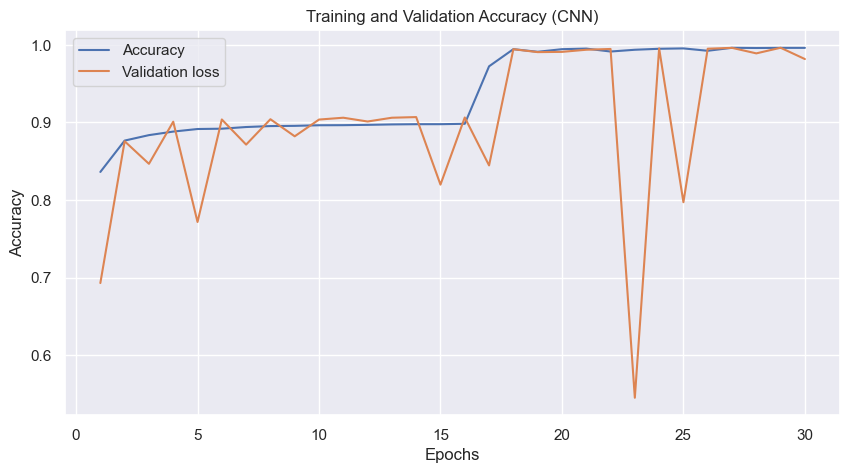
\includegraphics[width=400px]{figures/CNN_training_validation.png}
			\caption{Accuracy curve}
			\label{fig:aa}
		\end{figure}
		\begin{figure}[h]
			\centering
			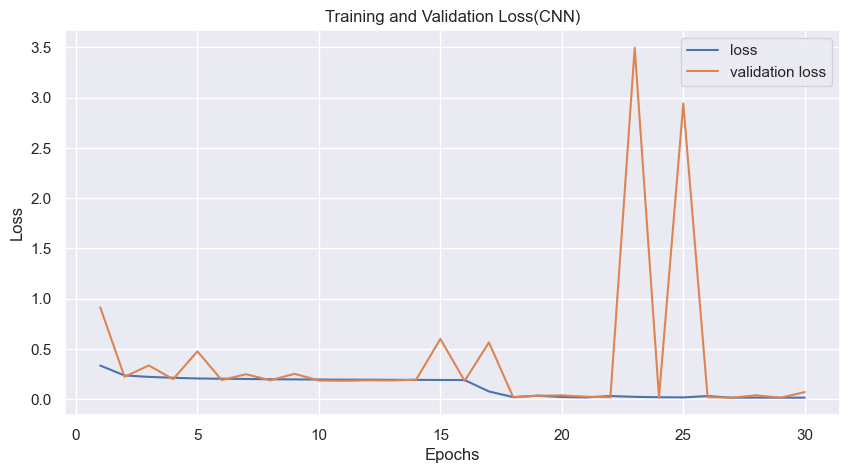
\includegraphics[width=400px]{figures/CNN_training_validation_loss.png}
			\caption{ Loss curve}
			\label{fig:ff}
		\end{figure}
		


\subsubsection{LSTM model}


evaluating the LSTM model with the test data:
\firmlist
		\begin{itemize}
			\item accuracy: 99.62\%
			\item loss: 1.6\%
		\end{itemize}

		% add recall precsition and f1-score
		% add confucsion matrix
		% images

		% show 3 last epochs 
		% show 2 graphs

		\begin{figure}[h]
			\centering
			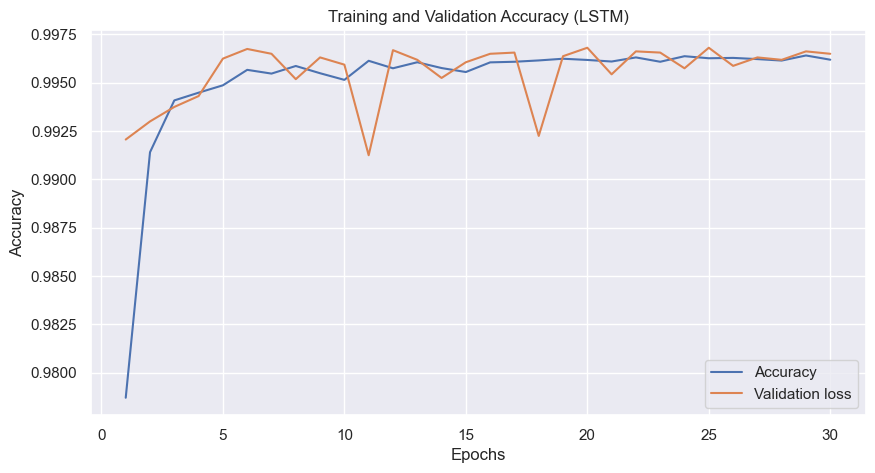
\includegraphics[width=400px]{figures/LSTM_training_validation.png}
			\caption{Accuracy curve}
			\label{fig:aa}
		\end{figure}
		\begin{figure}[h]
			\centering
			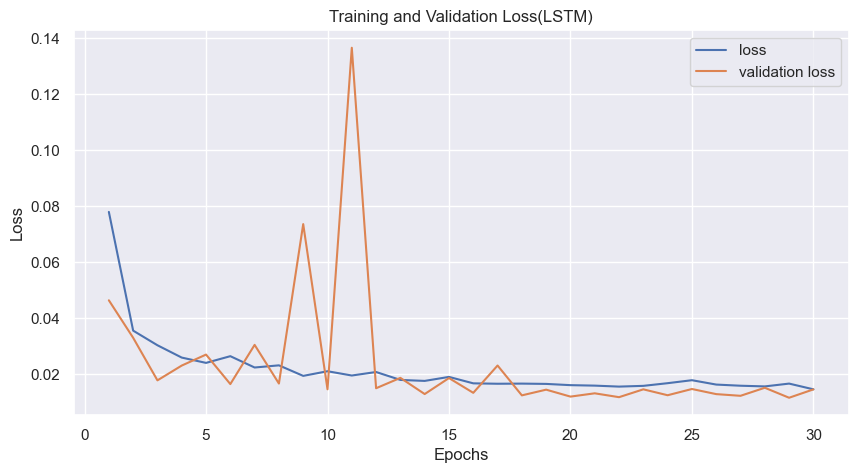
\includegraphics[width=400px]{figures/LSTM_training_validation_loss.png}
			\caption{ Loss curve}
			\label{fig:ff}
		\end{figure}
		





\paragraph{Observation}: We notice that the accuracy and the loss rates are almost matched between the CNN and the LSTM models. However according the validation accuracy compared to the number of epochs, the LSTM provides better accuracy over a wide rande of epochs(10 to 12 and 25 to30) unlike CNN which provides it's best accuracy over a narrow range of epochs(3 to 7 and 12 to 30).

		







\subsection{Conclusion}
In this chapter we demonstrated the development of two different deep learning methodes for creating a network intrusion detection system that protects the smart grid from DoS and DDoS attacks, starting with the development environment, the architecture of the used algorithms, and the data preprocessing, cleaning and training the models, and finishing the chapter with a performance comparison between the two models.





\newpage













	\chapter*{General Conclusion} \label{chap:conclusion}
\addcontentsline{toc}{chapter}{General Conclusion}





The proposed deep learning-based network intrusion detection system effectively addresses the issue of protecting smart grid infrastructure from Distributed Denial-of-Service (DDoS) attacks. The system leverages Convolutional Neural Networks (CNN) and Long Short-Term Memory (LSTM) algorithms to identify and prevent malicious traffic. This solution is particularly relevant in the context of smart grids, where the reliability and security of communication networks are crucial for efficient and safe operation.



\section*{contribution}


\begin{itemize}
    \item Development of a deep learning-based intrusion detection system: The system uses a combination of CNN and LSTM algorithms to identify DDoS attacks in smart grid communication networks.
    \item Improved accuracy and efficiency: The proposed system demonstrates enhanced accuracy and efficiency compared to traditional methods, making it a more effective solution for detecting and preventing DDoS attacks.
    \item Scalability and adaptability: The system is designed to be scalable and adaptable to various smart grid communication network configurations and traffic patterns.
\end{itemize}

    
    
\section*{Perspectives}

The applicability of this project is significant, as it can be integrated into existing smart grid infrastructure to enhance the security and reliability of communication networks. This can lead to improved overall performance and reduced downtime, ultimately benefiting both the grid operators and consumers. However, there are some limitations and perspectives to consider:


\section*{Limitations}
\begin{itemize}
    \item Data quality and availability: The quality and availability of training data can significantly impact the performance of the system. Future work should focus on developing methods to handle noisy or limited data.
    \item Real-time processing: The system's ability to process data in real-time is crucial for effective DDoS attack detection. Future improvements should focus on optimizing the system's processing speed and efficiency.
    \item Integration with existing systems: The system should be designed to seamlessly integrate with existing smart grid infrastructure and security systems to ensure a smooth transition and optimal performance.
    \item Future research directions: Future research should explore the application of other deep learning architectures and techniques to further improve the system's performance and adaptability.
\end{itemize}
    
    
    
    



By addressing these limitations and perspectives, the proposed deep learning-based network intrusion detection system can be further refined and optimized to provide enhanced security and reliability for smart grid communication networks.

	% \chapter{Template Items} \label{chap:template}

This part contains the typographical elements of the template, to be used in writing your Master's thesis. A course on scientific writing using \LaTeX{} is available at:
\url{https://drive.google.com/file/d/1coBxyvq-XRw5Sr3GO-VDJhYsPSLOQpRD/}
\\
\\
\textcolor{red}{
	This chapter aims to give you examples of the template. You must absolutely remove it during the final version of the thesis.
}

\section{Title - Level 2} \label{sec:example}
\subsection{Title - Level 3}
\subsubsection{Title - Level 4}

\section*{Title - Level 2 (Unnumbered)}
\subsection*{Title - Level 3 (Unnumbered)}
\subsubsection*{Title - Level 4 (Unnumbered)}

\section{Lists of Items}
This is normal text. followed by a list of items:

\firmlist
\begin{itemize}
	\item Item 1	
	\item Item 2
	\begin{itemize}
		\item Item A
		\item Item B
		\begin{itemize}
			\item Item I
			\item Item II
			\item ...
		\end{itemize}
	\end{itemize}
\end{itemize}

\noindent
And here is an enumerated list of items:

\begin{enumerate}
	\item Item 1	
	\item Item 2
	\begin{enumerate}
		\item Item A
		\item Item B
		\begin{enumerate}
			\item Item I
			\item Item II
			\item ...
		\end{enumerate}
	\end{enumerate}
\end{enumerate}

\section{Figures, Tables and Algorithms}
You can define several types of floating elements: Figures, tables, and algorithms.

\begin{figure}[h]
	\centering
	
\includegraphics[width=2.5cm]{figures/example}
	\caption{An example of figures}
	\label{fig:example} % label must always be after caption
\end{figure}

\begin{table}[h]
	\centering
	\caption{An example of tables}
	\begin{tabular}{|L{5.1cm}C{5.1cm}R{5cm}|}  % sum=15.2cm (L=Left, C=Center, R=Right)
	\hline
	Colonne 1 & Colonne 2 	 & Colonne 3 \\
	Ligne 1   & Ligne 1   	 & Ligne 1 	 \\
	Ligne 2   & Ligne 2 	 & Ligne 2 	 \\
	...	      & ... 		 & ... 		 \\
	...		  & ... 		 & ... 		 \\
	...		  & ... 		 & ... 		 \\
	\hline
\end{tabular}
	\label{tab:example} % label must always be after caption
\end{table}

\begin{algorithm}[h] 
	\selectlanguage{french}
	\begin{algorithmic}[1]
	\REQUIRE $i\in \mathbb{N}$
	\STATE $i\gets 10$
	\IF {$i\geq 5$} 
		\STATE $i\gets i-1$
	\ELSE
		\IF {$i\leq 3$}
			\STATE $i\gets i+2$
		\ENDIF
	\ENDIF 
\end{algorithmic}

%Documentation: https://mirror.marwan.ma/ctan/macros/latex/contrib/algorithms/algorithms.pdf

%\STATE <text>
%\IF{<condition>} \STATE {<text>} \ELSE \STATE{<text>} \ENDIF
%\IF{<condition>} \STATE {<text>} \ELSIF{<condition>} \STATE{<text>} \ENDIF
%\FOR{<condition>} \STATE {<text>} \ENDFOR
%\FOR{<condition> \TO <condition> } \STATE {<text>} \ENDFOR
%\FORALL{<condition>} \STATE{<text>} \ENDFOR
%\WHILE{<condition>} \STATE{<text>} \ENDWHILE
%\REPEAT \STATE{<text>} \UNTIL{<condition>}
%\LOOP \STATE{<text>} \ENDLOOP
%\REQUIRE <text>
%\ENSURE <text>
%\RETURN <text>
%\PRINT <text>
%\COMMENT{<text>}
%\AND, \OR, \XOR, \NOT, \TO, \TRUE, \FALSE
	\caption{An example of algorithms}
	\label{algo:example} % label must always be after caption
\end{algorithm}

\section{Cross-Referencing}

By using labels, it is possible to reference different elements of the document. As examples, Chapter \ref{chap:template}, Section \ref{sec:example}, Figure \ref{fig:example}, Table \ref{tab:example}, Algorithm \ref{algo:example} and Definition \ref{def:example}.


\begin{definition} \label{def:example}
	(Title of the definition)\\
	An example of definitions, $E=mc^2$...
\end{definition}

In addition to definitions, you can use theorems, proofs, remarks, notations, lemmas, or propositions.

\section{Source Codes}

You can also introduce source codes, like the following example which is written in Java language (The syntax highlighting can be customized in the file \texttt{"/macros.tex"}):

\begin{sourcecode}{/src/A.java}
	\lstinputlisting[language=Java]{listings/A.java}
\end{sourcecode}

\section{Bibliographic Citations}

References are managed using the Bib\TeX{} tool. The sources are stored and organized in the file \texttt{"bibliography.bib"}. To cite a source in the text, there are several possibilities:

\begin{itemize}
	\item \verb|\citet{bar73}| \quad $\Rightarrow$ \quad \citet{bar73} % Bardeen et al. [1973]
		\item \verb|\citep{bar73}| \quad $\Rightarrow$ \quad \citep{bar73} % [Bardeen et al., 1973]
	\item \verb|\citep[see][]{bar73}| \quad $\Rightarrow$ \quad \citep[see][]{bar73} % [see Bardeen et al., 1973]
	\item \verb|\citet*{bar73}| \quad $\Rightarrow$ \quad \citet*{bar73} % Bardeen, Carter, and Hawking [1973]
	\item \verb|\citep*{bar73}| \quad $\Rightarrow$ \quad \citep*{bar73} % [Bardeen, Carter, and Hawking, 1973]
	\item \verb|\citealt{bar73}| \quad $\Rightarrow$ \quad \citealt{bar73} % Bardeen et al. 1973
	\item \verb|\citeauthor{bar73}| \quad $\Rightarrow$ \quad \citeauthor{bar73} %  Bardeen et al.
	\item \verb|\citeauthor*{bar73}| \quad $\Rightarrow$ \quad \citeauthor*{bar73} % Bardeen, Carter, and Hawking
	\item \verb|\citeyear{bar73}| \quad $\Rightarrow$ \quad \citeyear{bar73} % 1973
	\item \verb|\citeyearpar{bar73}| \quad $\Rightarrow$ \quad \citeyearpar{bar73} % [1973]
\end{itemize} % To remove in final version


	%\chapter{Intrusion detection for smart grids}
	%\section{Introduction}
An intrusion detection system is a piece of hardware or software that is responsible for detecting suspicious and malicious activity, and in a network or an information system, the anomaly can either be reported to a systems administrator or saved to a security information and even management system (SIEM), the SIEM combines the output from multiple sources, then uses some filtering techniques to decide if the reported activity is malicious. \cite{1}Intrusion detection systems are categorized into 2 categories based on the location of the detection, which are either network or host-based (HIDS or NIDS), There are also two primary methods of intrusion detection: signature-based and anomaly-based. \cite{2}

	%\printbibliography
	
\backmatter
	\bibliographystyle{unsrtnat}
	\bibliography{bibliography}
	%\chapter*{Acronyms}
\addcontentsline{toc}{chapter}{Acronyms}

(You can list the acronyms used in the document, for example:)

\begin{acronym} 
	
	\acro{NTIC}{New Technologies of Information and Communication}
	\acro{UML}{Unified Modeling Language}
	IDS
	NIDS
	HIDS
	SIEM
	\acro{ADMS}{Advanced Distribution Management Systems}

	%\acro{}{}
	%\acro{}{}
	%\acro{}{}
\end{acronym} 

\end{document}